%%-------------------------process on a circle---------------------------------------%%
% \blue{
% 	discuss about data generation on a circle, 
% 	\begin{itemize}
% 		\item including circulant matrix
% 		\item why circulant matrix
% 		\item discuss covarince, biasness and the difficulties of estimation
% 		\item discuss variogram
% 		\item jones 1963
% 	\end{itemize}
% }

%%------------------------------------------------------------------%%
\section{Stationary process on a circle}
%%------------------------------------------------------------------%%

In this chapter we consider a real valued process $\{X(P): P\in S\}$ on the unit circle $S$, with finite second moment and continuity in quadratic mean. According to \cite{DUFOUR1976107} the process $\{X(P)\}$ can be represented in a Fourier series which is convergent in quadratic mean,

\beq
X(P) = A_0 + \sum_{n = 1}^\infty (A_n \cos(nP) + B_n \sin(nP).
\eeq


\begin{eqnarray}
	\nonumber
	\mbox{where} \quad A_0 &=&  \frac{1}{2\pi} \int_S X(P)dP, \\ \nonumber
	A_n &=& \frac{1}{\pi} \int_S \cos(nP)dP \\ 
	B_n &=& \frac{1}{\pi} \int_S \sin(nP)dP 
\end{eqnarray}

Let $P,Q$ be any two points on the circle, the covariance $R(P,Q)$ between the two points can be defined as,

\[
	R(P,Q) = E(X(P)X(Q)) = cov(X(P), X(Q))
\]

The process $X(P)$ is stationary if $E(X(P))$ is a constant and $R(P,Q)$ is function of the angular distance $\theta_{PQ}$ between $P$ and $Q$. If the process $X(P)$ is stationary on the circle,

\beq
cov(A_n, A_m) = a_n \delta(n,m) = cov(B_n, B_m), \quad \mbox{for $n, m \ge 0$}.
\eeq\\


Let $C(\theta), \theta \in [0, \pi ]$ denote a stationary covariance function on the circle, then

\beq
C(\theta) = \sum_{n=0}^\infty a_n \cos(n \theta),
\eeq

with $\sum_{n = 0}^\infty a_n < \infty$, and $a_n \ge 0$. Note that

\beq
a_n  =\frac{2}{\pi}\int_0^\pi C(\theta) \cos(n\theta)d\theta.
\eeq 




%%------------------------------------------------------------------%%
\section{Estimation}
%%------------------------------------------------------------------%%


Let $\{X(t_k)\}$ be a collection of gridded observations on a circle, with $t_k = (k-1)*2\pi/n, k = 1, 2, \cdots, n$. Lets assume $E(X(t)) = \mu$ is unknown, and estimated by $\bar{X} = \frac{1}{n}\sum_{i=1}^{n} X(t_i)$. The underlying process is stationary, if it's covariance function solely depends on the distance $\theta$,
\beq
C(\theta) = cov(X(t_k+\theta), X(t_k)), \quad \quad \theta \in [0, \pi].
\eeq


The gridded points $\{X(t_k)\}$ on a circle can be represented as $\utilde{X} = (X_1, X_2, \cdots, X_n)^T$ and the variance-covariance matrix of the sample vector $\utilde{X} $ is given by $\Sigma$. Further, we can denote $\bar{X}$ in the following form,
\[
	\bar{X} = \frac{1}{n}{\bf 1}_n^T \utilde{X}
\]

\begin{eqnarray}
	\mbox{then,} \quad var(\bar{X}) &=& cov(\frac{1}{n}{\bf 1}_n^T \utilde{X}, \frac{1}{n}{\bf 1}_n^T \utilde{X}) \nonumber \\
	&=& \frac{1}{n^2}{\bf 1}_n^T \Sigma {\bf 1}_n \nonumber \\
	&=& \frac{1}{n} \left(C(0)+C(\pi)+2 \sum_{m=1}^{N-1}C(m 2\pi/n)\right) \nonumber
\end{eqnarray}

When $n \to \infty$, (assuming $C(\theta)$ is a continuous function on $[0, \pi]$)
%is integrable, or more strongly,
\[
	\frac{1}{n} \left(2 \sum_{m=0}^{N}C(m 2\pi/n)\right) = \frac{1}{\pi} \frac{\pi}{N} \left( \sum_{m=0}^{N}C(m 2\pi/n)\right) \to \frac{1}{\pi} \int_0^\pi C(\theta)d\theta = a_0.
\]

\begin{eqnarray*}
	\mbox{Hence} \quad	var(\bar{X}) &=& \frac{1}{n} \left(2 \sum_{m=0}^{N}C(m 2\pi/n)\right) - \frac{1}{n}(C(0) + C(\pi)) \\
	&\to & a_0, \quad \quad \mbox{as $n \to \infty$}.
\end{eqnarray*}

 
\[
	\mbox{We can conclude that}	var(\bar{X}) \to \frac{1}{\pi} \int_0^\pi C(\theta)d\theta \quad \mbox{as $n \to \infty$}.  
\]


\begin{prop}
	
	Mean of the gridded points $\bar{X}$ is not a consistent estimator for $\mu$, mean on a circle. 
	
	\[
		P(|\bar{X} - \mu| > \varepsilon) \to 0.
	\]  
	
	If $var(\bar{X}) \to 0$, then from Chebyshev's inequality we have 
	
	\[
		P(|\bar{X} - \mu| > \varepsilon) \le \frac{var(\bar{X})}{\varepsilon^2} \to 0, \quad \mbox{for any $\varepsilon > 0$}.
	\]
	
	Therefore, $var(\bar{X}) \to 0$ is a sufficient condition for consistency, but it is not necessary. However, if we assume $\utilde{X}$ is multivariate normally distributed, then $\bar{X}$ follows normal distribution with mean $\mu$ and approximate variance $a_0$. Then ($Z \sim N(0, 1)$)
	\begin{eqnarray*}
		P(|\bar{X} - \mu| > \varepsilon) = P\left(\frac{|\bar{X} - \mu|}{\sqrt{a_0}} > \frac{\varepsilon}{\sqrt{a_0}}\right) \approx P\left(|Z| > \frac{\varepsilon}{\sqrt{a_0}}\right) \not\to 0  
	\end{eqnarray*}
	since $\frac{\varepsilon}{\sqrt{a_0}}$ is a fixed constant for each fixed $\varepsilon > 0$.\\
	
\end{prop}

%-------------------------------------% 
\subsection{Estimation of covariance on a circle} \label{est_covariance}
%-------------------------------------%

We used method of moments (MOM) to estimate the covariance $C(\theta)$ on a circle, the estimator can be given by

\beq \label{covarince_estimator}
\hat{C}(\Delta \lambda) = \frac{1}{n}\sum_{i = 1}^n (X(t_i + \Delta \lambda) - \bar{X})(X(t_i) - \bar{X}), 
\eeq

where $\Delta \lambda = 0, 2\pi/n, 4\pi/n, \cdots, 2(N-1)\pi/n$.\\

We can show that the above estimator is a biased estimator for $C(\theta)$ .

\begin{eqnarray}
	\nonumber
	E(\hat{C}(\Delta \lambda)) &=& \frac{1}{n}\sum_{i = 1}^n E((X(t_i + \Delta \lambda) - \bar{X})(X(t_i) - \bar{X})) \\ \nonumber
	&=& \frac{1}{n}\sum_{i = 1}^n E((X(t_i + \Delta \lambda) - \mu - (\bar{X} - \mu))(X(t_i) -\mu - (\bar{X}) - \mu)) \\ \nonumber
	&=& \frac{1}{n}\sum_{i=1}^n cov(X(t_i+\Delta \lambda), X(t_i)) - \frac{1}{n}\sum_{i = 1}^n E((X(t_i + \Delta \lambda) - \mu)(\bar{X} - \mu)) \\ \nonumber
	& & -\frac{1}{n}\sum_{i = 1}^n E((X(t_i) - \mu)(\bar{X} - \mu)) + \frac{1}{n}\sum_{i = 1}^n E((\bar{X} - \mu)(\bar{X} - \mu)) \\ \nonumber
	&=& C(\Delta \lambda) -E((\bar{X} - \mu)(\bar{X} - \mu)) - E((\bar{X} - \mu)(\bar{X} - \mu)) \\ \nonumber 
	& & + E((\bar{X} - \mu)(\bar{X} - \mu)) \\ \nonumber
	&=& C(\Delta \lambda) - var(\bar{X}).
\end{eqnarray}

% Moreover,
% 
% \begin{eqnarray*}
% 	\nonumber
% 	var(\bar{X}) &=& E((\bar{X} - \mu)(\bar{X} - \mu)) = \frac{1}{n^2}\sum_{i = 1}^n \sum_{j=1}^n E(X(t_i) - \mu)(X(t_j) - \mu) \\ \nonumber
% 	&=&  \frac{1}{n^2}\sum_{i = 1}^n \sum_{j=1}^n cov(X(t_i), X(t_j)) = \frac{1}{n^2}\sum_{i = 1}^n \sum_{j=1}^n C(m*(i-j)*2\pi/n) \\ \nonumber
% 	&=& \frac{1}{n^2}\sum_{i = 1}^n \sum_{j=1}^n \left(a_0 + \sum_{k=1}^\infty a_k \cos(m*(i-j)*2\pi/n)\right) \\ \nonumber
% 	&=& a_0 + \sum_{k=1}^\infty a_k \left(\frac{1}{n^2}\sum_{i = 1}^n \sum_{j=1}^n \cos(m*(i-j)*2\pi/n)\right).
% \end{eqnarray*}
% 
% Now,
% 
% \begin{eqnarray*}
% 	& & \sum_{i = 1}^n \sum_{j=1}^n \cos(m*(i-j)*2\pi/n) \\
% 	&=& \sum_{i=1}^n \sum_{j=1}^n \left(\cos(m*i *2\pi/n)\cos(m*j*2\pi/n) + \sin(m*i *2\pi/n)\sin(m*j*2\pi/n) \right)\\
% 	&=& \left(\sum_{i=1}^n \cos(m*i *2\pi/n)\right)^2 + \left(\sum_{i=1}^n \sin(m*i *2\pi/n)\right)^2 = n^2
% \end{eqnarray*}
% 
% since for any integer $m$, we have
% 
% \[
% 	\sum_{k = 1}^{n} \cos(mk*2\pi/n) = \left\{\begin{array}{cc}
% 	0, & \mbox{for any integer $m \ne 0$,}  \\
% 	n, & \mbox{for $m = 0$}
% 	\end{array}
% 	\right. \mbox{ and }
% 	\sum_{k = 1}^{n} \sin(mk*2\pi/n) = 0.
% \]
% 
% Hence,
% \[
% 	var(\bar{X}) = a_0.
% \]
% 
% Therefore,
% \beq
% E(\hat{C}(\Delta \lambda)) = C(\Delta \lambda) - a_0.
% \eeq



% {\bf Note}: When $var(\bar{X}) \not\to 0$, we can not make the conclusion that $\bar{X}$ is not consistent. For consistency, we need to prove that


{\bf Remark 1} The MOM estimator $\hat{C}(\Delta \lambda)$ of the covariance function is actually a biased estimator with the shift amount of $a_0$. Therefore, if $a_0 = 0$ for a covariance function, we have the unbiased estimator $\hat{C}(\Delta \lambda)$. \\

{\bf Remark 2} If the gridded points were on a line, for example in time series, $E(\bar{X} - \mu)^2 \to 0$ as $n \to \infty$ under the assumption that the covariance function $C(\theta) \to 0$ when $\theta \to \infty$ (which is practically feasible), that is, $\bar{X}$ is consistent in the case of points on a line. In the case of circle, we might not have $C(\theta)$ close to 0 since $\theta$ is within a bounded region ($(0, \pi)$ for the circle) and we normally assume $C(\theta)$ is continuous for $\theta$. \\


%-------------------------------------%
\subsection{Estimation of variogram on a circle}
%-------------------------------------%

The theoretical variogram function is given by,
\beq
\gamma(\theta) = C(0) - C(\theta).
\eeq
and the MOM estimator for the variogram is given by,

\beq
\hat{\gamma}(\Delta \lambda) = \frac{1}{2n} \sum_{i=1}^n (X(t_i + \Delta \lambda) - X(t_i))^2.
\eeq

We can show that variogram estimator through MOM is an unbiased estimator, 

\begin{eqnarray*}
	E(\hat{\gamma}(\Delta \lambda)) &=& \frac{1}{2n} \sum_{i = 1}^n E(X(t_i + \Delta \lambda) - X(t_i))^2 \\
	&=& \frac{1}{2n} \sum_{i = 1}^n E((X(t_i + \Delta \lambda)-\mu) - (X(t_i) - \mu))^2 \\
	&=& \frac{1}{2n} \sum_{i = 1}^n cov(X(t_i + \Delta \lambda) - X(t_i), X(t_i + \Delta \lambda) - X(t_i)) \\
	&=& \frac{1}{2n} \sum_{i = 1}^n \left\{ cov(X(t_i + \Delta \lambda), X(t_i + \Delta \lambda)) + cov(X(t_i), X(t_i)) \right. \\
	& & \left. - 2cov(X(t_i + \Delta \lambda), X(t_i)) \right\}\\
	&=& \frac{1}{2n} \sum_{i = 1}^n \left( C(0) + C(0) - 2C(\Delta \lambda)\right) \\
	&=& C(0) - C(\Delta \lambda) = \gamma(\Delta \lambda).
\end{eqnarray*}
 
\blue{need to prove consistency}


%-------------------------------------%
\section{Data generation on a circle}
%-------------------------------------% 



First, we will discuss how to generate correlated data at $n$ girdded points on a circle when the covarince function is defined and compare above covariance and variogram estimators. Since the observed data are correlated, the covariance function can be written as a function of distance (angle). For simplicity we will use exponential family covarince function as given below, 

\beq \label{exp_covarince} 
C(\theta) = C_1e^{-a|\theta|},
\eeq

where $\theta = i*\Delta\lambda = \pm i*2\pi/n, i=1,2,\cdots,n/2$\\

\begin{figure}
	\centering
	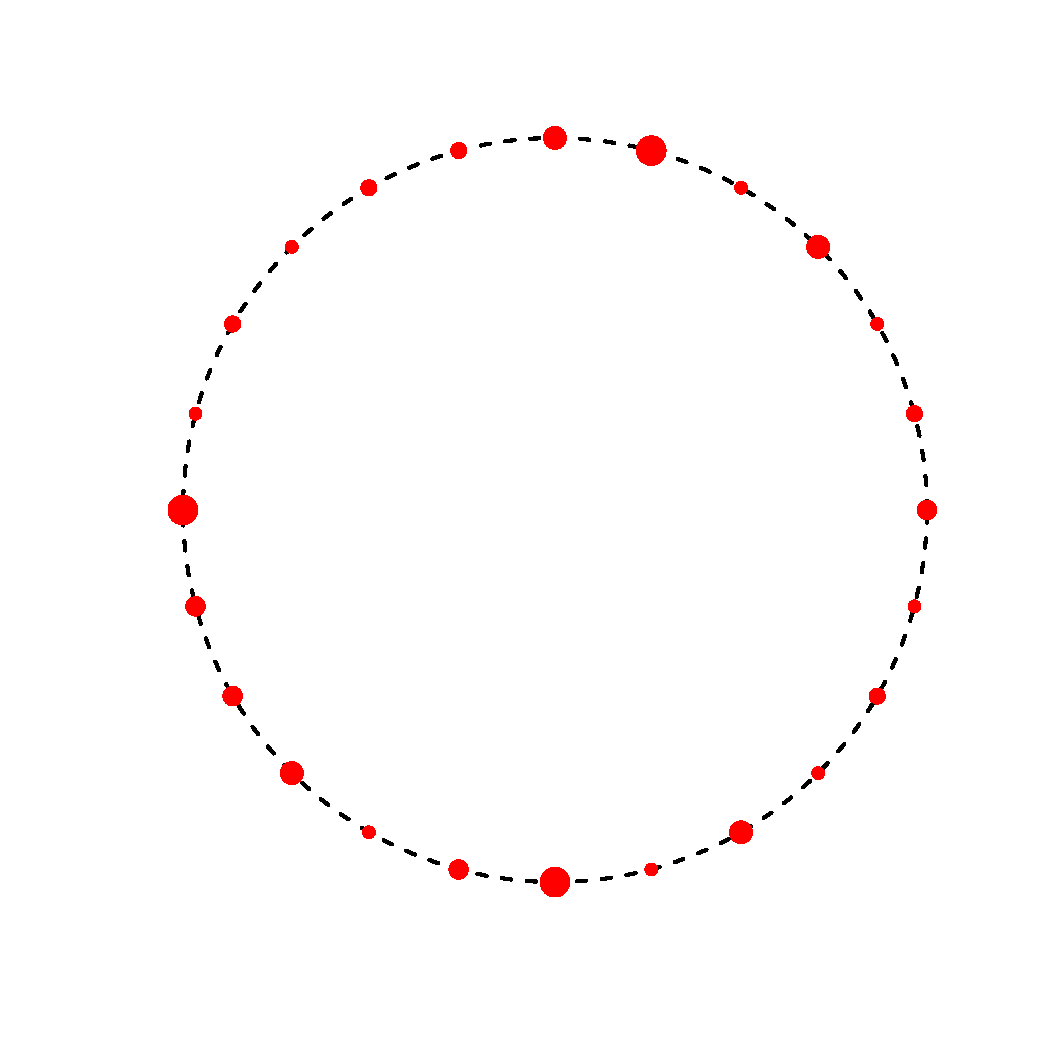
\includegraphics[width=0.5\textwidth]{graphs/process_circle}
	\caption {Random process on a circle at 24 points ($\Delta\lambda = 15^0$), the red dots represent the  observed values at a given time and each point is associated with a random process of it's own.}
\end{figure}

Clearly, each location is correlated with other $n-1$ locations and $C(\theta) = C(-\theta)$ the variance-covariance matrix $\Sigma$ is circulant and will be in the following form,   


\begin{eqnarray*}
	\Sigma &=& circ(C(0),C(\delta), C(2\delta), \cdots, C((N-1)\delta), C(\pi),  C((N-1)\delta), \cdots, C(\delta)) \\
	&=& \left(\begin{array}{ccccccc}
	C(0)      & \cdots & C((N-1)\delta ) & C(\pi) &  C((N-1)\delta ) & \cdots & C(\delta) \\
	C(\delta) & \cdots & C((N-2)\delta) & C((N-1)\delta) &  C(\pi)  & \cdots & C(2\delta) \\
	C(2\delta) & \cdots & C((N-3)\delta) & C((N-2)\delta) &  C((N-1)\delta) & \cdots & C(3\delta)\\
	\vdots    & \vdots  & \vdots  & \vdots  & \vdots  & \vdots  & \vdots  \\
	C(\delta) & \cdots & C(\pi) &  C((N-1)\delta) & C((N-2)\delta)  & \cdots & C(0) 
	\end{array} \right) \\
	&=& Q\Lambda Q^T,
\end{eqnarray*}

where $\delta = 2\pi/n,\ \Lambda=\{\lambda_1, \lambda_2,\cdots,\lambda_n\}$ and $Q=\{\psi_1, \psi_2,\cdots,\psi_n\}$ are the respective eigen values and eigen vectors of the above circulant matrix. Now using singular value decomposition (SVD) we can obtain the correlated data $\utilde{X}$ on a circle as follows,

\[
	\utilde{X} = \Sigma^{1/2}*Z = Q\Lambda^{1/2}Q^T*Z 
\]

where $Z\sim N(\utilde{0},1_{n})$.

%-------------------------------------%
\subsection{Compare covariance estimator} 
%-------------------------------------%

% \beq\label{cov:circle1}
% C(\theta) = \frac{1}{n_L} \sum_{i=1}^{n_L} (X(a_i+\theta)\cdot X(a_i))-(\overline{X(a)})^2
% \eeq
\begin{itemize}
		
	\item Using the exponential covariance function given by \ref{exp_covarince}
	      	      
	      In section \ref{est_covariance} we proved that, in general the covarince estimator (\ref{covarince_estimator}) on a circle is biased, with a bias of $var(\bar{X})$. In order to compare this estimator to it's theoretical covarince given by equation \ref{exp_covarince}. We computed the MOM estimator $\hat{C}(\theta)$ with 48 gridded observations on the circle from 500 simulations. 
	      	      
	      \begin{figure}[H] 
	      	\label{covarince_circle}
	      	\centering
	      	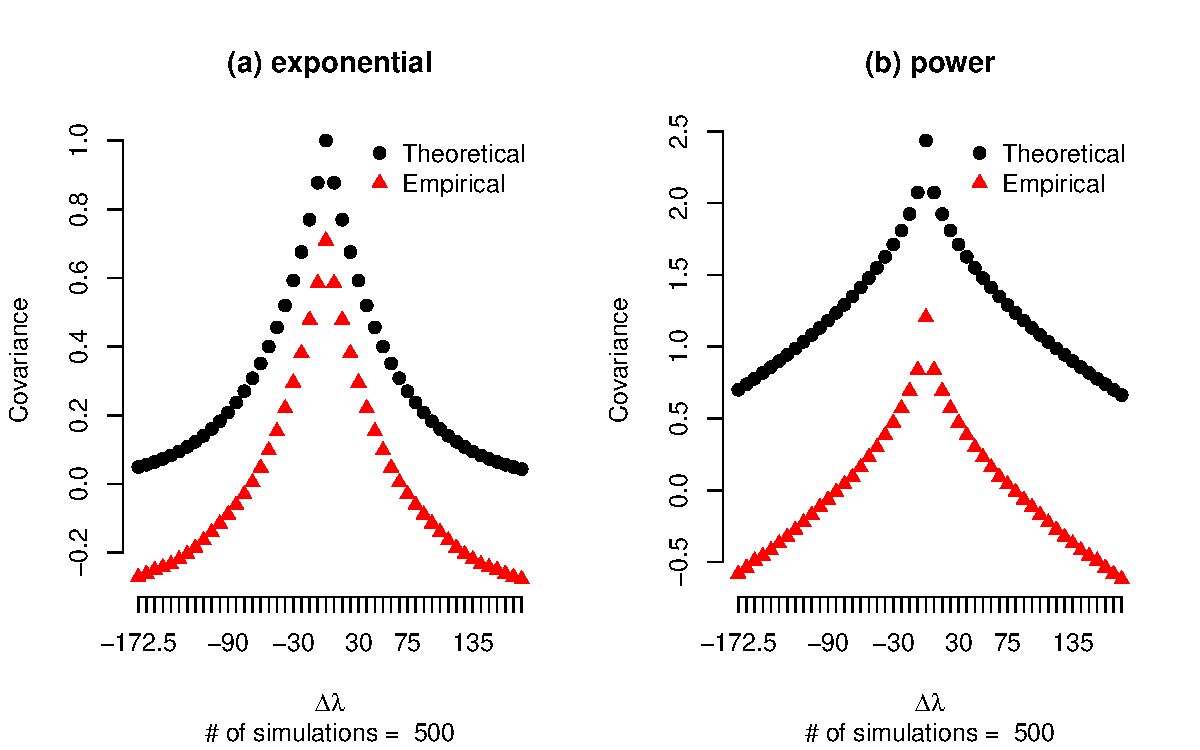
\includegraphics[width=0.65\textwidth]{graphs/covarince_circle}
	      	\caption {Theoretical and empirical covariance (with bias) comparison on a circle}
	      \end{figure}
	      	      
	      {\bf Remark 1} We have noticed that the shift between theoretical and empirical values were approximately equal to $a_0$.\\
	      	      
	      % \blue{should we talk about $\hat{var(\bar{X})} = var(\bar{X}_1, \cdots, \bar{X}_k) $??, $a_0 = 0.3045545 \quad \hat{var(\bar{X})}$ will be close to  $a_0$ as we increase the number of simulations }
	      
	      % and this cannot be estimated since there is only one data point at each location
	      	      
	\item However, we can obtain $a_0$ for the above exponential covarince as follows,
	      \[
	      	a_0 = \frac{C_1}{a\pi}(1 - e^{-a\pi})
	      \]
	      	      
	      We consider the following covariance function, after subtracting $a_0$ from $C(\theta)$. The theoretical and empirical values match perfectly.
	      \[
	      	D(\theta) = C(\theta) - a_0.
	      \]
	      	      
	      % \beq \label{cov:circle1}  
	      % C(\theta) = \frac{1}{n_L} \sum_{i=1}^{n_L} (X(a_i+\theta) \cdot X(a_i)) 
	      % \eeq
	      	      
	      \begin{figure}[H]
	      	\centering
	      	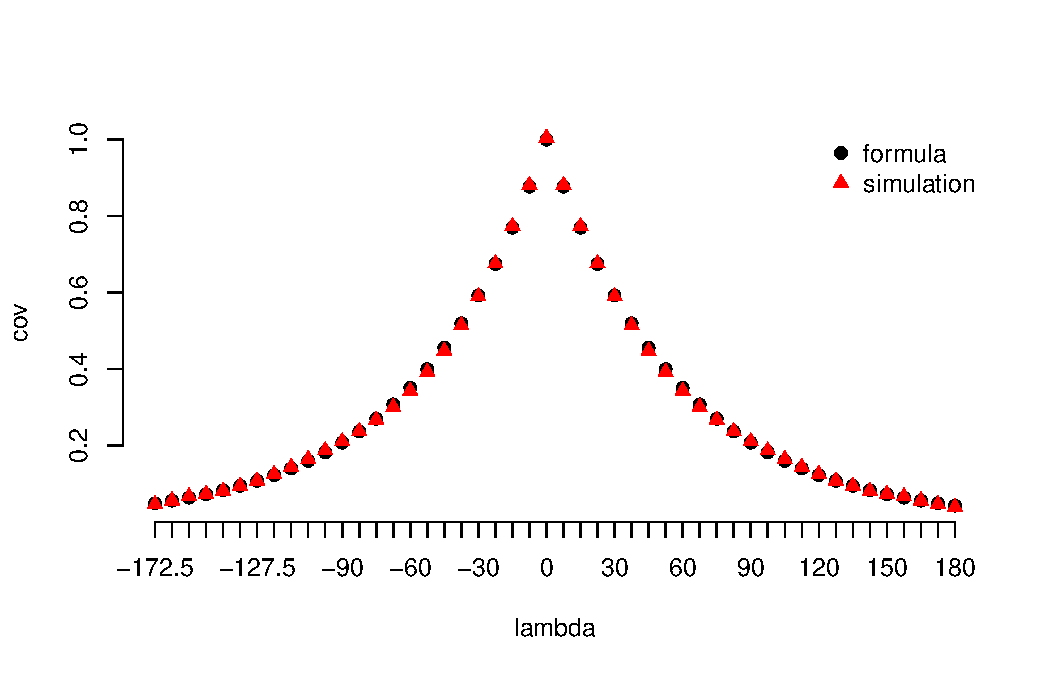
\includegraphics[width=0.65\textwidth]{graphs/Summary-covarince_circle_2}
	      	%graph from data genaration summary doc line 194 
	      	\caption {Theoretical and empirical covariance comparison on a circle}
	      \end{figure}
	      	      
	      Note, if the process is a zero mean process the covariance estimator will be unbiased ($i.e. Var(\bar{X}) = 0$) hence we will get a perfect match between theoretical and empirical values.
	      	      
\end{itemize}

%-------------------------------------%
\subsection{Compare variogram estimator} 
%-------------------------------------%

We proved that in general the variogram estimator is unbiased \blue{and consistentcy}. The theoretical variogram based on exponential covariance is given below,   

\[
	\gamma(\theta) = C(0) - C(\theta) = C_1(1-e^{-a|\theta|})
\]

Again we computed the variogram estimator $\hat{\gamma}(\theta)$ with 48 gridded observations on the circle from 4000 simulations and there is a perfect match between theoretical and empirical values.


\begin{figure}[H]
	\centering
	%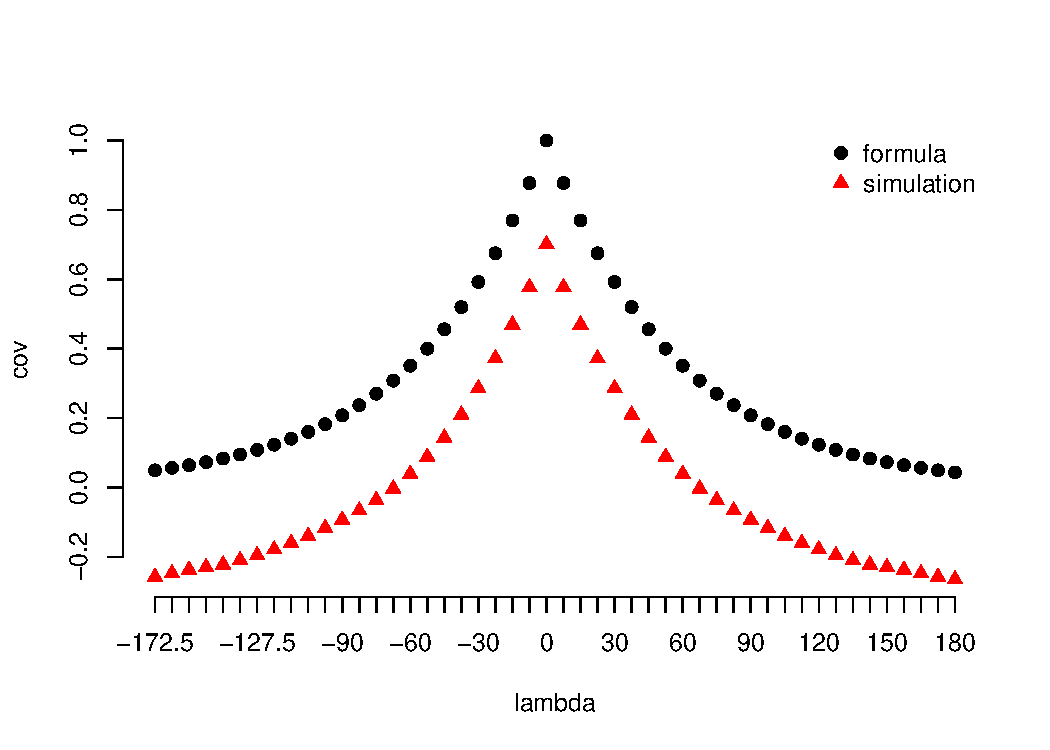
\includegraphics[width=0.65\textwidth]{graphs/Summary-covarince_circle_1}
	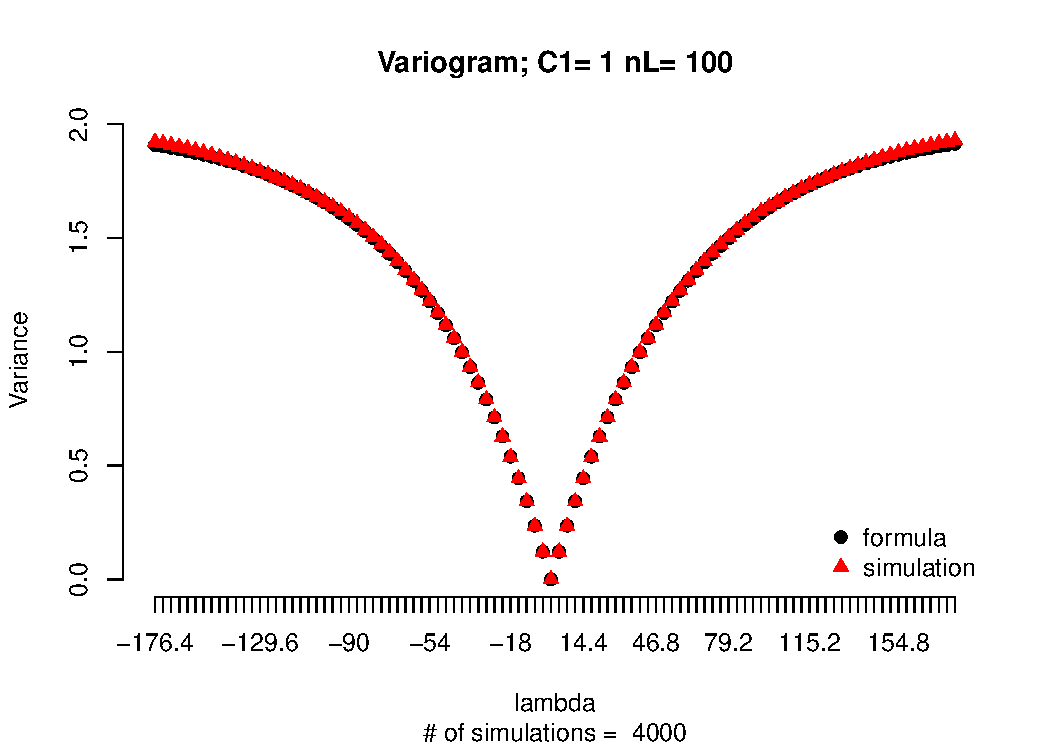
\includegraphics[width=0.65\textwidth]{graphs/variogram_plot_4000}
	%graph from data genaration summary doc line 177 
	\caption {Theoretical and empirical comparison for variogram on a circle}
\end{figure}


